% !TEX root = main.tex
\section{Obecna implementacja modułu AthenaMonitoring}
Dotychczas środowisko Athena używało jednowątkowego przetwarzania algorytmów. 
Ich sekwencja wykonania jest z góry określona przez pliki konfiguracyjne napisane w Pythonie. 
Służą one również do wystartowania całego zadania, np. rekonstrukcji. 
Algorytmy współdzielą dane poprzez pisanie i odczytywanie ich ze wspólnego magazynu danych (Event Store). 
Mogą one również używać narzędzi, które są konfigurowane niezależnie. 
Algorytmy mogą wchodzić w interakcję z serwisami, których cykl życia jest niezależny od cyklu wykonania algorytmów.
W kontekście monitoringu, najważniejszy jest serwis do histogramowania (THistSvc), który zajmuje się zapisywaniem histogramów ROOT na dysk. 
Schemat wykonania rekonstrukcji został pokazany na \figref{fig:athena:oldFlow}.

\begin{figure}[!ht]
\centering
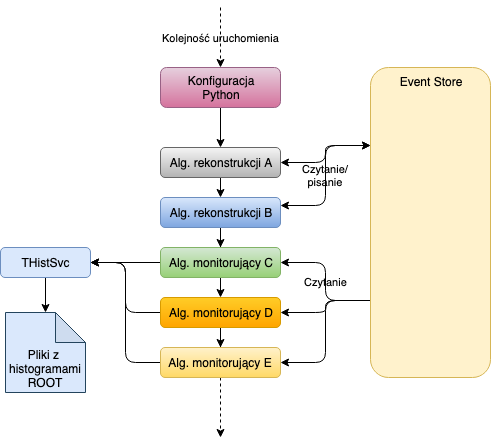
\includegraphics[width=0.75\textwidth]{img/old_flow.png}
\caption{
Schemat prezentuje proces wykonania kodu w aktualnej implementacji środowiska Athena. 
Kolejność algorytmów jest sztywno zdefiniowana w pliku konfiguracyjnym, w którym algorytmy monitorujące wykonywane są po algorytmach rekonstrukcji, które te dane produkują. 
Następnie algorytmy monitorujące komunikują się z serwisem THistSvc w celu zapisania gotowych histogramów do plików ROOT.
}
\label{fig:athena:oldFlow}
\end{figure}

\comment{
\begin{itemize}
\item co istniało do tej pory?
\item czemu potrzeba czegoś nowego?
\item wady starego rozwiązania
\item czemu monitoring jest ważny?
\item do czego jest używany?
\item na co pozwalał dotychczas?
\item WYDAJNOŚĆ
\item BEZPIECZEŃSTWO dla wielowątkowości
\item kto używa kodu, dostosowanie do klienta
\item co to Athena, gdzie jest uzywana, do czego, co to CERN, ile danych przetwarza
\item czemu nowe rozwiązanie pomoże unikać pomyłek w danych wejściowych!!!
\item co to algorytmy i filtrowanie ONLINe i OFFLINE
\item data quality
\end{itemize}
}